\documentclass[12pt]{article}
\setlength{\textwidth}{17cm}
\setlength{\textheight}{24cm}
\setlength{\topmargin}{-2cm}
\setlength{\footskip}{1cm}
\setlength{\evensidemargin}{0cm}
\setlength{\oddsidemargin}{0cm}
\setlength{\parindent}{0cm}

\usepackage{allrunes}
\usepackage{amsmath}
\usepackage[magyar]{babel}
\usepackage[T1]{fontenc}
\usepackage[utf8]{inputenc}
\usepackage{fixltx2e}
\usepackage{multirow}
\usepackage{mathtools}

\usepackage[hyphens]{url}
\usepackage[unicode,colorlinks=true,breaklinks]{hyperref}
%\usepackage[dvips]{hyperref}
%should display links, but it does not work with \H accent
%and formulas in section titles

\hypersetup{colorlinks,linkcolor=blue,urlcolor=magenta,citecolor=magenta}
%Breaks long url`s in text, while keeping it one link:

\usepackage{amsfonts}
\usepackage{amsthm}
\usepackage{amssymb}

\theoremstyle{plain}
\usepackage{graphicx}

%\usepackage{gensymb}
\usepackage{float}

% For bra-ket notation
\usepackage{braket}


\begin{document}
\title{9. tétel \\ Képfeldolgozás}
\author{Bulatovic Nikola}

\maketitle

\pagenumbering{gobble}

\begin{abstract}
    Képek digitális reprezentációja, színmodellek. Interpolációs, konvolúciós és dekonvolúciós módszerek, homomorf szűrés. Élek, sarkok és foltok detektálása. Morfológiai analízis, jellemzők kinyerése. Perspektívakorrekció, zajszűrési módszerek. \\ \par
    Ez a tétel főként a \textit{Digitális képfeldolgozás} kurzus alapján készült, ami nagyrészt a \textit{Digital Image Processing} című könyv \cite{img_proc} tematikáját követi. A kurzushoz a Fizweben is található egy jegyzet \cite{fizweb}. Egyéb felhasznált jegyzetek \cite{gepi_latas,kepelemzes_magyar}. A tétel tematikájában  bőven akad olyan téma, ami nem szerepelt a kurzuson még említés szintjén sem, így nem hiszem, hogy elvárás ezek részletes ismerete. Ezek a témakörök vagy egyáltalán nem szerepelnek az említett forrásokban, vagy egy nagyon hosszú, részletesen kidolgozott fejezet, ami ebben a tételben nem fejthető ki. Ezek a fejezetek általánosan kerülnek bemutatásra, egy nagy képet próbálnak adni a témáról. A legfontosabb témakörök (digitális reprezentáció, szűrők,  képjavítás, képrekonstrukció, színmodellek) már nagyobb részletességgel vannak kifejtve.  
\end{abstract}

\vfill

\tableofcontents

\newpage
\section{Képek digitális reprezentációja}

\begin{itemize}

\item Egy kép egy $f: (x,y) \mapsto f(x,y)$ kétváltozós függvénnyel reprezentálható, ahol $x$-et és $y$-t \textit{térbeli} (spatial) koordinátáknak, $f(x,y)$-t pedig  az adott pontbeli  \textit{intenzitásnak} vagy amplitúdónak nevezzük. Ha a kép valamilyen fizikai folyamat által generált, akkor $f(x,y)$ arányos a forrás által sugárzott és/vagy visszavert fénnyel. 

\item A kép a térbeli koordinátákban és az amplitúdóban is folytonos (a képet rögzítő különböző hardverek/szenzorok kimenete általában folytonos feszültségjel). Ahhoz, hogy \textit{digitális}, azaz a térbeli koordinátákban és az amplitúdóban diszkrét értékeket felvevő képet kapjunk, két eljárás szükséges (\ref{fig:sampling}. ábra). A koordináták digitalizálását mintavételezésnek (sampling), az amplitúdókét pedig kvantálásnak (quantization) hívjuk. A digitális képek így véges számú elem, \textit{pixel} együtteséből áll.

\item Többféle intenzitás skála lehetséges, pl.: bináris (fekete-fehér), 8-bites grayscale. A 8-bites szürkeskálájú, és monokromatikus (egyféle frekvenciát tartalmazó) képek esetén az intenzitásértékek a 0 - 255 (fekete - fehér) között vesznek fel valamilyen egész értéket, amelyhez egy szürke szín tartozik \cite{grayscale}. Létezik még 12-, 16-bites, illetve tetszőleges lehetséges értékű lebegőpontos skálák is. Színes kép (pl.: RGB) esetén egy pixelhez három érték tartozik (lsd. Színmodellek fejezet).  




\begin{figure}[H]
    \begin{center}
    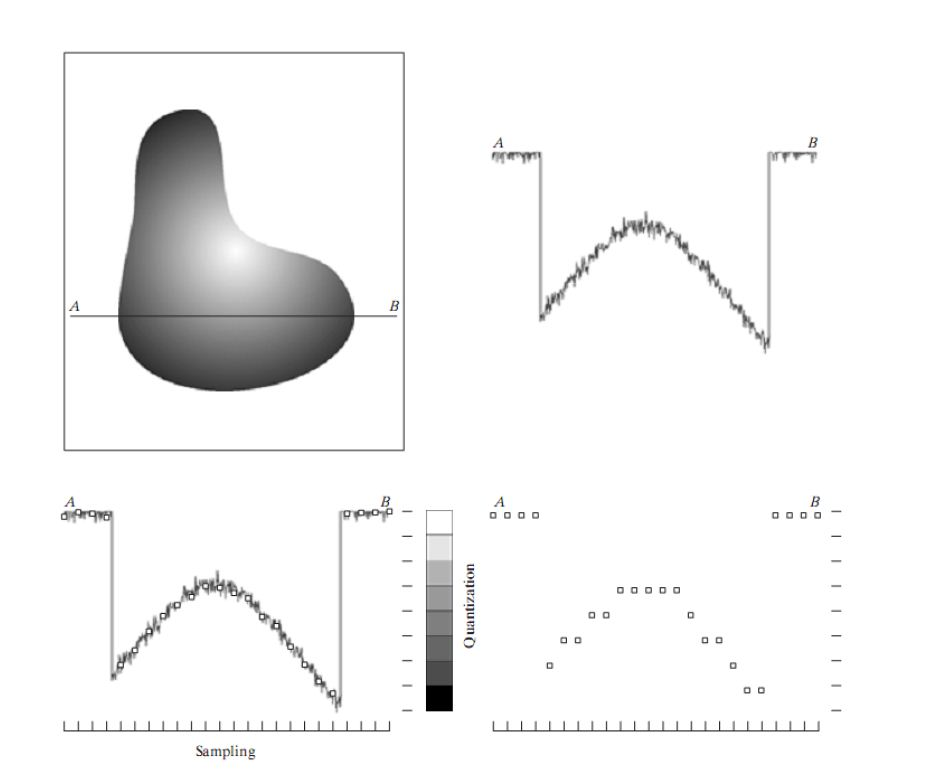
\includegraphics[width=0.75\linewidth]{media/sampling.JPG}
    \caption{\textbf{Képek digitalizációjának folyamatai.} A folytonos kép - az AB egyenes által kijelölt - sorát egyenlő méretű mintákra osztjuk (sampling). Ezután a mintavételezett függvény amplitúdóit diszkretizáljuk (quantization). A teljes digitalizáció eredménye egy 2 dimenziós mátrix.} 
    \label{fig:sampling}
    \end{center}
\end{figure}

\item A képtérben (spatial domain) végzett különböző műveletek általában nagy számításigényűek, ezért gyakran használjuk a frekvenciatartományt (frequency domain). A kettő között a Fourier-transzformáció teremt kapcsolatot, melynek 2 dimenziós, $N \times M$ méretű, diszkrét kép esetén alakja a következő:
$$\mathcal{F}(f(x,y)) = F(u,v) = \frac{1}{MN}\sum^{M-1}_{x=0}\sum^{N-1}_{y=0}f(x,y)e^{-2\pi i(\frac{ux}{M} + \frac{vy}{N})}$$
$$\mathcal{F}^{-1}(F(u,v)) = f(x,y) = \sum^{M-1}_{u=0}\sum^{N-1}_{y=0}F(u,v)e^{2\pi i(\frac{ux}{M} + \frac{vy}{N})}.$$

\end{itemize}{}
%%%%%%%%%%%%%%%%%%%%%%%%%%%%%%%%%%%%%%%%%%%%%%%%%%%%%%%%%%%%%

%%%%%%%%%%%%%%%%%%%%%%%%%%%%%%%%%%%%%%%%%%%%%%



\section{Szűrések}
\subsection{Szűrések a képtérben - konvolúció}
\begin{itemize}
\item A képfeldolgozás egy tipikus feladata a képjavítás (image enchancement), azaz a kép vizuális megjelenésének javítása. Egy ilyen feladat történhet képtérben és frekvenciatérben is. A képtérben végzett tipikus műveletek az ún. maszkprocesszálások, ezeket képtérbeli szűrésnek (spatial filtering) is nevezik. Léteznek még pontprocesszálások is (kontraszt javítás, hisztogram módosítás), de ezek nem szerepelnek a tétel a tematikájában.
\item A maszk (másnéven ablak vagy kernel) alapú transzformációk esetében a kép egy adott pixelét a környezetében lévő pixelek függvényében módosítjuk: $g(x,y) = T[f(x,y)]$, ahol $T$ egy lokális művelet, a szomszédos pixelekre hat. Fontos, hogy pontról pontra haladunk a transzformáció során, és nem írjuk önmagába az eredményt.
\item A legegyszerűbb, lineáris esetben a pixel értéke a környezetének valamilyen lineáris kombinációja. Ekkor a transzformációt szokás konvolúciós maszkolásnak, vagy csak konvolúciónak nevezni.
\item Az elnevezés abból ered, hogy a maszkprocesszálás művelete felfogható az eredeti kép ($f(x,y)$), és egy $m \times n$ méretű ablak ($w(x,y)$) 2 dimenziós, diszkrét konvolúciójának:
$$g(x,y) = w(x,y) * f(x,y) = \sum^a_{s = -a}\sum^b _{t=-b}w(s,t)f(x-s,y-t),$$
ahol $a = (m-1)/2$ és $b = (n-1)/2.$
\item Példák maszkokra:
\begin{itemize}
\item[-] Elmosás/simítás (átlagolás): $1/9 \begin{pmatrix} 
1 & 1 & 1 \\
1&1 & 1 \\
1 & 1 & 1
\end{pmatrix}$
\item[-] Él kiemelés (ha átmegy egy él $\neq 0$, egyébként $=0$): $\begin{pmatrix} 
-1 & -1 & -1 \\
-1&8 & -1 \\
-1 & -1 & -1
\end{pmatrix}$
\end{itemize}{}
\item A konvolúció egy nevezetes tulajdonsága, hogy két függvény konvolúciójának Fourier-transzformáltja megegyezik a Fourier-transzformáltak szorzatával:
$$f(x,y) * g(x,y) \Longleftrightarrow F(u,v)G(u,v)$$
\end{itemize}{}

\subsection{Szűrések a frekvenciatérben}
\begin{itemize}
\item Ha a kép mérete $N^2$ a maszké $n^2$, akkor $\sim N^2 \cdot n^2$ műveletet kell elvégezni, ami meglehetősen számításigényes. A frekvenciatérben az alacsony frekvenciás komponensek a képtér lassú változású részeinek felelnek meg, a magas frekvenciájú komponensek pedig a gyorsan változó részeknek. Ötlet: csináljuk meg az előző transzformációkat (simítás, élkiemelés) a frekvenciatérben.
\item Végezzük el a kép Fourier-transzformációját. Ezután, ha csak az alacsonyfrekvenciás komponenseket hagyjuk meg, akkor simítást végzünk. Ehhez a össze kell szoroznunk a szűrőt és a transzformált képet, majd az eredményt visszatranszformálni (\ref{fig:filter}. ábra).
\item Az ideális aluláteresztő szűrő: $H(u,v,D_0) =$    $\left\{
\begin{array}{ll}
      1 & \sqrt{u^2 + v^2} < D_0 \\
      0 & \sqrt{u^2 + v^2} \geq D_0 \\
\end{array} \right.$
\item A konvolúció tulajdonsága miatt ez a transzformáció megegyezik azzal, mintha konvolváltuk volna az eredeti  képet az ideális szűrő Fourier transzformáltjával. Így a normál tér és a Fourier tér közötti kapcsolat:

$$G(u,v) = H(u,v)F(u,v)$$
$$g(x,y) = h(x,y) * f(x,y),$$

ahol $g(x,y)$ és $G(u,v)$ az eredmény kép illetve annak Fourier-transzformáltja. A $h(x,y)$-et válaszfüggvénynek (point-spread function, PSF) nevezzük, mivel a Green-függvényhez hasonló módon megadja az egységimpulzusú gerjesztésre (itt egy fényes pontot jelent a sötét hátteren) adott választ. Ennek Fourier-transzformáltját $H(u,v)$-t válaszfüggvénynek hívjuk. 

\item Az ideális szűrő alakjában lévő éles letörések miatt a Fourier-transzformáltban magasabb komponensek is megjelennek, az eredmény nem lesz jó („szellemkép”). Ezért nem szokás használni ideális szűrőt, hanem helyette például a Butterworth-szűrőt:
$$H(u,v,D_0) = \frac{1}{1+[ \sqrt{u^2 + v^2}/D_0]^{2n} },$$
ahol n paraméter kontrollálja a függvény simaságát: $n\rightarrow \infty$ esetén visszakapjuk az ideális szűrőt.  

\item Magasfrekvenciás komponenseket meghagyva az eljárás teljesen hasonló, csak így felüláteresztő szűrőket kapunk, amelyekkel az éleket tudjuk kiemelni. 
\item A frekvenciatérben számolva a teljes transzformáció kevésbé számításigényes, továbbá a Fourier-transzformáció két változóban való szeparálhatósága miatt párhuzamosítható a feladat, illetve használható a Fast Fourier-transformation (FFT). 

\begin{figure}[H]
    \begin{center}
    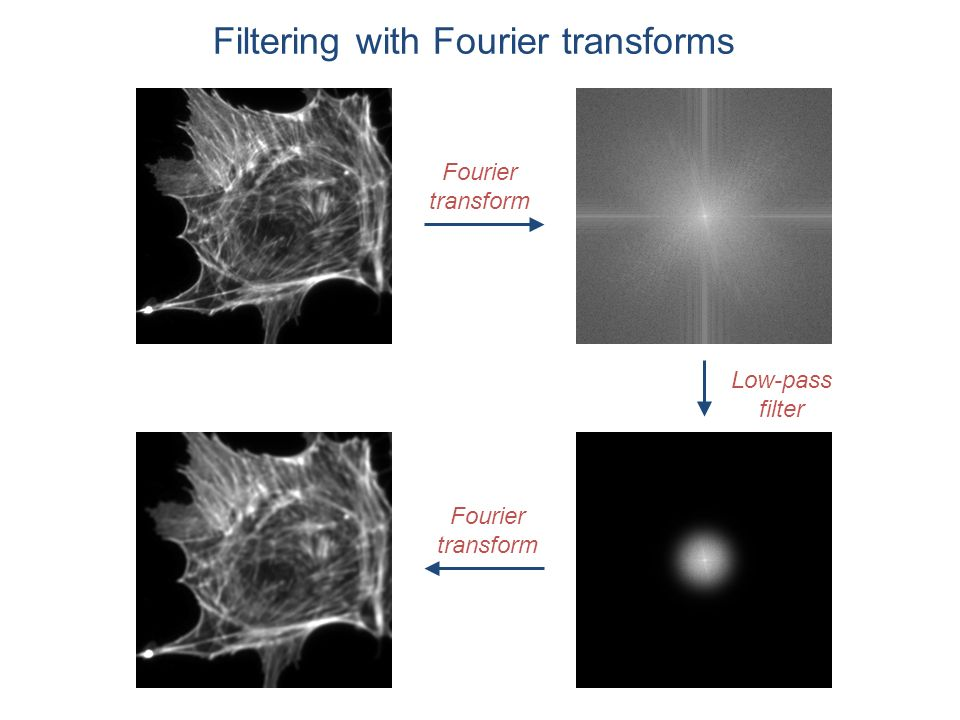
\includegraphics[width=0.75\linewidth]{media/filter.jpg}
    \caption{\textbf{Élsimítás aluláteresztő szűrővel frekvencia tartományban.} Megjegyzés: a szűrő láthatóan nem ideális, a vágási frekvenciánál ($D_0$) a függvény elég sima.} 
    \label{fig:filter}
    \end{center}
\end{figure}

\end{itemize}{}

\subsection{Homomorf szűrés}

\begin{itemize}
\item Léteznek egyéb nemlineáris szűrési technikák, mint például a homomorf szűrés. Ez az eljárás nemlineáris módon képezi le a képet a frekvenciatérbe, ahol lineáris szűrési technikák alkalmazása után visszaképződik az eredeti képtérbe.

\item Egy $f(x,y)$ kép felbontható két komponens szerint: a kép forrásának fénye (illumunitaion), illetve a képen szereplő objektumok visszaverődése (reflectance) szerint a következő módon: 
$$f(x,y) = i(x,y)r(x,y).$$
$$0 < f(x,y) < \infty$$
$$0 < i(x,y) < \infty$$
$$0 < r(x,y) < 1$$

\item Ezeken a komponenseken így nem tudunk műveleteket végezni a frekvenciatérben, mert a Fourier-transzformáltakra nem áll fent egyenlőség: $$\mathcal{F}[f(x,y)] \neq \mathcal{F}[i(x,y)]\mathcal{F}[r(x,y)].$$
\item Vegyük a két komponens logaritmusát, majd ezeket transzformáljuk:
$$Z(u,v) \vcentcolon=\mathcal{F}[ln(f(x,y))] =\mathcal{F}[ln(i(x,y))]+\mathcal{F}[ln(r(x,y))].$$
\item Ezeken tetszőleges $H(u,v)$ frekvenciatérbeli szűrőt használhatunk, majd ezt transzformáljuk vissza:
$$s(x,y) \vcentcolon= \mathcal{F}^{-1}[H(u,v)Z(u,v)] =  \underbrace{\mathcal{F}^{-1}[H(u,v)\mathcal{F}[ln(i(x,y))]]}_{i'(x,y)} + \underbrace{\mathcal{F}^{-1}[H(u,v)\mathcal{F}[ln(r(x,y))]]}_{r'(x,y)}.$$
\item Az eredmény exponenciálisát véve adódik a filterezett eredménykép:
$$g(x,y) = e^{i'(x,y)}e^{r'(x,y)} = i_0(x,y)r_0(x,y).$$

\item Homomorf szűréssel egyidejűleg lehet normalizálni a fényerőt és növeli a kontrasztot, mivel a két komponens szeparálva van: a homomorf szűrő függvény így külön hat ezekre. A $i$ komponenst lassú, az $r$ komponenst gyors változás jellemzi a képtérben, ezért egy olyan szűrőt kell alkalmazni, amely különböző módon kontrollálja a magas és alacsony frekvenciás komponenseket. Ilyen homomorf szűrő például általánosított Gauss felüláteresztő szűrő (\ref{fig:gauss}. ábra).

\begin{figure}[H]
    \begin{center}
    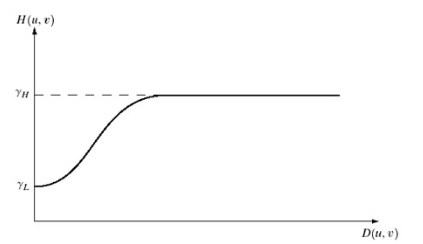
\includegraphics[width=0.75\linewidth]{media/gauss.png}
    \caption{\textbf{Homomorf felüláteresztő szűrő.} A szűrő két paramétere $\gamma_L,\gamma_H$ kontrollálja az alacsony és magas frekvenciás komponenseket. $D(u,v,) $ az origótól való távolságot jelenti a frekvenciatérben.} 
    \label{fig:gauss}
    \end{center}
\end{figure}


\end{itemize}{}

\section{Képrekonstrukciós módszerek}

\begin{itemize}
    \item Az előzőekben említésre került a képjavítás. Ennek a célja az volt, hogy a kép minőségét javítva vizuálisan jobb képet eredményezzen (kontraszt növelése, simítás, stb.). Ezeknek a módszereknek egyfajta szubjektív eredményeik voltak.
    \item A képrekonstrukció során ezzel szemben valamilyen priori tudásunk van a kép degradációját okozó jelenségről (pl.: egy autóból lett fényképezve és elmosódott). A képrekonstrukció célja a degradáció matematikai modellezése és annak megszüntetése. Rekonstrukciós módszerek pl.: inverz szűrés, zajszűrés, stb. Ezek eredménye már objektíven mérhető. Megjegyezendő, hogy a két módszer között vannak átfedések.
    \item A degradáció általános modellje a következő:
    $$\underbrace{g(x,y)}_{\text{eredmény kép}} = \underbrace{H[f(x,y)]}_{\text{degradált eredeti kép}} + \underbrace{\eta(x,y)}_{\text{zaj}}$$
\end{itemize}{}

\subsection{Zajszűrési módszerek}

\begin{itemize}
    \item Speciális esetként tegyük fel, hogy a $H$ operátor az identitás. Ekkor csak a zajból eredő torzításokkal kell foglalkozni.
    \item A kép létrehozása során számtalan helyen léphetnek különböző eredetű zajok.
    \item A zajok lehetnek függetlenek a térbeli koordinátáktól, azok független valószínűségi változóként kezelhetőek adott eloszlással (pl.: gauss, egyenletes, impulzusok). Ezen kívül lehetséges periodikus zajok is.
    \\
    \item Tisztán additív zajok esetén az előzőekben ismertetett képtérbeli szűrők alkalmazhatók:
    \begin{itemize}
        \item[-] Különböző átlagok (számtani, geometriai)
        \item[-] Medián
        \item[-] Max/min, stb.
    \end{itemize}{}
    \item Periodikus zajok esetén a frekvenciatérbeli szűrések használhatók:
    \begin{itemize}
        \item[-] Sávvágó (bandreject) szűrő: bizonyos frekvencia tartományt nem enged át. Ha ismert a zaj körülbelüli frekvenciája. 
        \item[-] Sáváteresztő (bandpass) szűrő: az előző ellentetje. 
        \item[-] Notch szűrők: adott frekvenciák körüli tartományban átereszt vagy vág.
    \end{itemize}{}
\end{itemize}{}

\subsection{Dekonvolúciós módszerek}

\begin{itemize}
    \item A dekonvolúciós problémák is az előző degradációs egyenlet speciális esetei: amikor a $H$ operátor egy adott függvénnyel való konvolúciót jelöl, azaz frekvenciatérben:
    $$G(u,v) = H(u,v)F(u,v) + N(u,v),$$
    ahol $N(u,v)$ a zaj Fourier-transzformáltját jelöli.
    \item Ennek a problémának megoldása egy olyan X filter megtalálása, amelyre:
    $$X(u,v)[H(u,v)F(u,v) + N(u,v)] = D(u,v) ,$$
    és $ F \approx D.$
    \item Számos dekonvolúciós módszer létezik \cite{deconv}:
    \begin{itemize}
        \item[-] Inverz szűrő dekonvolúció: Ha feltesszük, hogy $H$ ismert és $N = 0$, ekkor $X(u,v) = H^{-1}(u,v)$. A gyakorlatban ez gyenge közelítés, már minimális zaj tönkreteszi a dekonvolúciót és nem kapjuk vissza az eredeti képet.
        \item[-] Regularizált inverz: $X$ alakja hasonló az előzőhöz, de egy adott értéknél levág. Az előzőnél már robosztusabb a hibákra. $X(u,v) =$    $\left\{
        \begin{array}{ll}
          H^{-1}(u,v) & |H^{-1}(u,v)| \leq t \\
          t & |H^{-1}(u,v)| > t \\
        \end{array} \right.$
        \item[-] Wiener szűrő: Minimalizálja $|F-D|$ várható értékét, a zaj összes realizációjára, Gaussos fehér zajt feltételezve.
        \item[-] Maximum A Priori algoritmus (MAP): nemlineáris, bayesi módszer.
    \end{itemize}{}
\end{itemize}{}




\section{Élek, sarkok és foltok detektálása}
\begin{itemize}
    \item Megjegyzés: ez a témakör meglehetősen szerteágazó és nem triviális. A legalapvetőbb dolgok felületes leírása is megsokszorozná a tétel hosszát, illetve ezek a témakörök nem szerepeltek a kurzuson, csak említés szintjén. Ebben a fejezetben ezért \cite{el} alapján csak egy kvalitatív, nagy kép következik a témakörről.

    \item A keresett alakzatok (\ref{fig:edges}. ábra) definíciói a következők:
    \begin{itemize}
        \item[-] Él: a képfüggvény intenzitás-gradiense nagy valamely irányban. 
        \item[-] Sarkok: Két él találkozása, minden irányban nagy intenzitásváltozás.
        \item[-] Foltok: Egy kompakt régió.
    \end{itemize}{}
    
    \item A képfüggvény deriváltja egy adott pontban mutatja a legnagyobb csökkenés irányát, ami merőleges az élre (ha van az adott pontban), illetve a gradiensvektor nagysága jellemzi az él erősségét.
    \item A képen éleket lehet az első- vagy másodrendű deriváltak számításával keresni. Mindkettő nagyon zajérzékeny, ezért célszerű előzőleg képsimítást végezni a zaj hatásának csökkentésére.
    \item Mivel a digitális képek diszkrétek, ezért a deriváltszámítás is diszkrét lesz. Jellemzően X- és Y-irányú parciális deriváltakat közelítünk konvolúciós kernelekkel.

    \item A simító és parciális deriváltat közelítő konvolúciók általában összevonhatók közös kernelbe, így egy lépésen végrehajthatók.

    \item Egy jól használható éldetektor további feltételezésekkel is él, ilyen például a Canny detektor (simítás, deriválás, nem maximális élek elnyomása, hiszterézis küszöbölés).
    
    \item Foltok detektálásához is konvolúciós módszereket használnak általában, azonban ezek sokkal bonyolultabbak az élek detektálásánál.
    
\end{itemize}{}


\begin{figure}[H]
    \begin{center}
    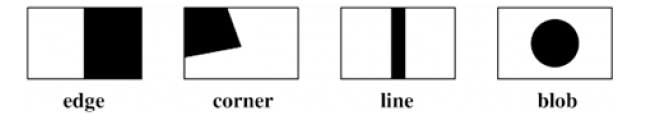
\includegraphics[width=0.75\linewidth]{media/edges.png}
    \caption{\textbf{A képfeldolgozásban leginkább használt lokális képi sajátosságok.} Él, sarok, vonal, folt.} 
    \label{fig:edges}
    \end{center}
\end{figure}

\section{Morfológiai analízis, jellemzők kinyerése}

\begin{itemize}
    \item A morfológia szó eredete állatok, növények, vagy szavak struktúra- és alakelemzése. A képfeldolgozásban hasonló módon strukturáló elemekkel történő struktúra- és alakelemzést jelent.
    \item A képet "összeütköztetjük" csúsztatott strukturáló elemmel, ezáltal kifejezőbb alakra hozva.
    \item Definíciók:
    \begin{itemize}
        \item[-] $B$ strukturáló elem: adott műveletre szánt diszkrét ponthalmaz egy $c$ origóval
        \item[-] $X$: Bemeneti bináris kép
        \item[-] $B_X$: $B$ olyan transzlációja (pozíciója), hogy az origója x pontban van. A művelet eredményét egy kimeneti képbe írjuk, nem X-be.
    \end{itemize}{}
    \item A legtöbb morfológiai művelet két műveleten keresztül fejezhető ki:
     \begin{itemize}
        \item[-] Erózió $X\ominus B$: A művelet eredménye $1$, ha $B$ minden pontja egybe esik $X$ valamely pixelével, egyébként 0.
        \item[-] Dilatáció $X\oplus B$: A művelet eredménye $1$, ha $B$ legalább egy pontja egybe esik $X$ valamely pixelével, egyébként 0.
    \end{itemize}{}
    \item Ezekből további műveletek generálhatók, amely (\ref{fig:morf}. ábra):
    \begin{itemize}
        \item[-] Zárás: $(X\oplus B) \ominus B$
        \item[-] Nyitás: $(X\ominus B) \oplus B$
    \end{itemize}{}   
    \item Ezeken kívüli egyéb műveletek alkalmasak pl.: sarokkeresésre, határkiemelésre, középvonal megtalálására.
\end{itemize}{}

\begin{figure}[H]
    \begin{center}
    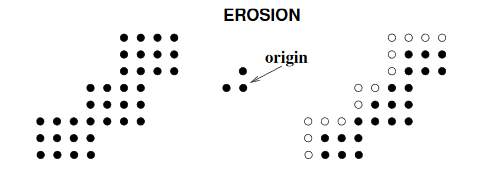
\includegraphics[width=0.65\linewidth]{media/er.png}
    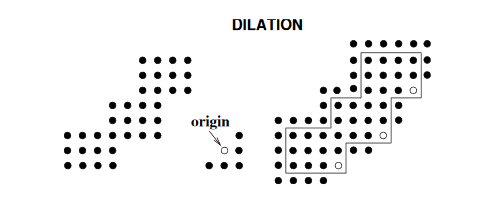
\includegraphics[width=0.65\linewidth]{media/dil.png}
    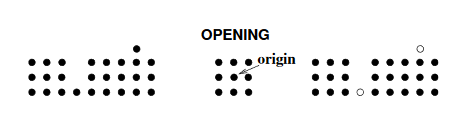
\includegraphics[width=0.65\linewidth]{media/open.png}
    
\includegraphics[width=0.65\linewidth]{media/clos.png}
    \caption{\textbf{Morfológiai műveletek.} A két alapművelet az erózió és dilatáció. A strukturáló elemek az ábrák közepén láthatók. Az ezekből konstruált nyitás a kontúrokat simítja el, a zárás pedig kitölti a keskeny réseket.} 
    \label{fig:morf}
    \end{center}
\end{figure}



\section{Perspektívakorrekció}
\begin{itemize}
    
\item A perspektívakorrekciós eljárások olyan transzformációk, amelyek a perspektívikus hatások hibáit próbálja korrigálni. Perspektíváról akkor beszélünk, amikor az adott kép mélységgel is rendelkezik. Ekkor a képen lévő objektumok olyan módon torzulnak, hogy a kamera forrához közelebb lévők nagyobbnak, a távolabbiak kisebbnek tűnnek. 

\item A perspektíva hatása könnyen észlelhető egy négyzetes hálón: ha megmérjük a négyzetek pixel mértetét, azt tapasztaljuk, hogy az a távolság függvényében csökken. Ez problémákat okoz, mivel bármilyen méret/távolság mérésnél figyelembe kell venni ezt az effektust.

\item a perspektívakorrekciós algoritmusok gyakorlatilag egy forgatást végeznek az eredeti képen, úgy, hogy az elforgatott kép úgy néz ki, mintha fentről egyenesen letekintenénk a képre, nem pedig egy adott szöget bezárva azzal (\ref{fig:pers}. ábra). Ilyen módon a különböző alakzatok alakja és távolsága a képen megegyezik a valós alakkal és mérettel.

\end{itemize}{}

\begin{figure}[H]
    \begin{center}
    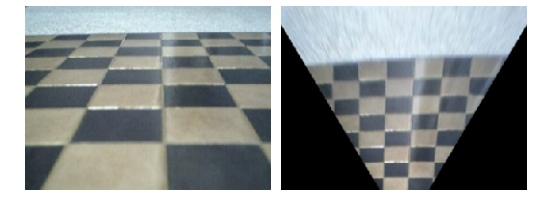
\includegraphics[width=0.75\linewidth]{media/p1.png}
    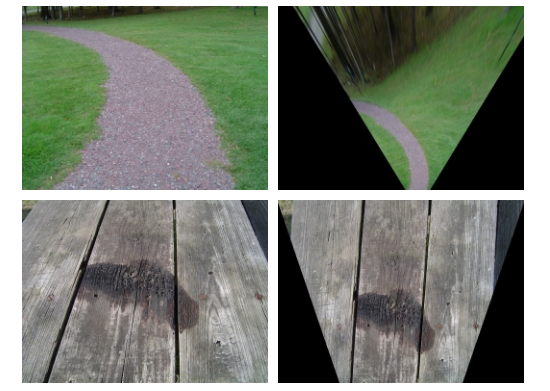
\includegraphics[width=0.75\linewidth]{media/p2.png}
    \caption{\textbf{Példák a perspektíva korrekciójára.} Láthatóan a korrigált négyzetek mérete és alakja megegyezik.} 
    \label{fig:pers}
    \end{center}
\end{figure}




\section{Interpoláció}

\begin{itemize}
    

\item Az interpoláció alapvető eszköz olyan feladatokban, mint nagyítás, kicsinyítés, forgatás. Az interpolálás egy újramintavételezési (resampling) folyamat, melyben ismert adatpontokból becsüljük meg a más helyen lévő, nem ismert függvényértékeket. A következőkben a nagyítás példáján keresztül nézzük ezt meg, hiszen alkalmazása is itt a leggyakoribb.

\item Legyen egy $500 \times 500$ pixel méretű kép, amit $750 \times 750$-es méretre szeretnénk nagyítani. Képzeletben vegyünk egy $750 \times 750$-es rácsot, amit lezsugorítunk a kép eredeti méretére. A lekicsinyített rács pixelei sűrűbben fognak elhelyezkedni, az eredeti kép pixeleihez képest. Ezekhez a pixelekhez kell valamilyen módon értéket rendelni, majd visszanagyítva megkapjuk az eredeti kép nagyított változatát (\ref{fig:int}. ábra). 

\begin{figure}[H]
    \begin{center}
    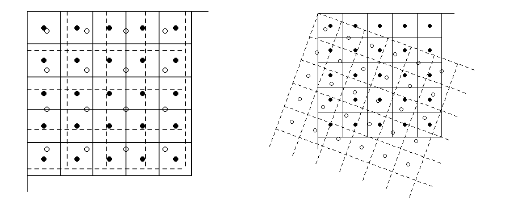
\includegraphics[width=0.75\linewidth]{media/interpol.png}
    \caption{\textbf{Példa kép kicsinyítésére és forgatására.} A folytonos fekete vonal az eredeti kép, a szaggatott pedig a transzformált. Az üres körökben nem ismerjük a kép intenzitását.} 
    \label{fig:int}
    \end{center}
\end{figure}


\item A pixelek intenzitásértékének kiszámításához többféle módszer létezik.
\begin{itemize}

\item[-] Legközelebbi szomszéd interpoláció: az ismeretlen pixel értékének a legközelebbi ismert pixel értékét adjuk. Ez a legegyszerűbb, de ritkán használt eljárás, mivel pl. torzításokat okozhat.

\item[-] Bilineáris interpoláció: ha $v(x,y)$ a keresett, ismeretlen intenzitás, akkor
$$v(x,y) = ax +by +cxy +d, $$
ahol az $a,b,c,d$ paraméterek a négy legközelebbi szomszédból határozhatóak meg.

\item[-] Bicubic interpoláció: hasonló módon az előzőhöz az első 16 legközelebbi szomszéd alpaján határozza meg az intenzitást. 

\item[-] Léteznek még több szomszédot felhasználó eljárások, és egyéb szofisztikált technikák (spline, wavelet). Ezek pontosabbak, mint az előzőek, de nyilván számításigényesebbek is. A standard, legtöbbet használt általános célú eljárás a bicubic módszer. A legtöbb képszerkesztő programban is ezt használják pl.: Adobe Photoshop.
\end{itemize}
\end{itemize}{}

\section{Színmodellek}
\begin{itemize}
    \item Az elektromágneses spektrum kb. $435 - 700 nm$-es sávja a látható fény tartománya. Az emberi szemben a csapok úgy működnek, mint a színszűrők, és ezek csúcsai 3 fő szín: a piros, zöld, kéknek megfelelő hullámhossznál vannak. Trikromatikus látásunk van, azaz alapvetően három színnel dolgozik, ezekből további színek kombinálhatóak.
    \item 1931-ben a CIE szervezet definiálta a három elsődleges szín (RGB) pontos hullámhosszát.
    \item Két elsődleges szín keverékéből jönnek ki a másodlagos színek, mindháromból pedig a fehér szín. Az RGB additív színmodellből a kevert színek komponensei a következő módon számíthatóak:
    $$x = \frac{X}{X+Y+Z},$$
    $$y = \frac{Y}{X+Y+Z},$$
    $$z = \frac{Z}{X+Y+Z},$$
    $$x+y+z = 1,$$
    
    ahol $X,Y,Z$ a három színhez tartozó intenzitás.
    
    \item A lehetséges színek ábrázolásának hasznos módja a kromacitás diagram felrajzolása. Mivel egy színt két független változó határoz meg a diagrammot csak az $xy$ síkban szokás ábrázolni. A diagram használata azért kényelmes, mert bármely két szín keveréke a két színt összekötő szakasz felezőjén van. Az $x=y=1/3$ pontban található a fehér pont. Egy szín ettől való távolsága S (szaturáció) adja meg a szín élénkségét. Az ún. H (hue) polárszög érték adja meg a szín fajtáját.  A gammut a kromacitás diagramm egy részhalmazát adja meg. A legnagyobb gammut a látható fénytartomány által körbekerített teljes diagramm.
    
    
    \begin{figure}[H]
    \begin{center}
    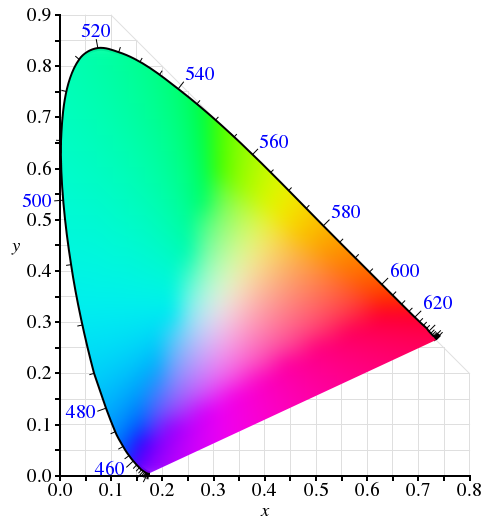
\includegraphics[width=0.55\linewidth]{media/chro.png}
    \caption{\textbf{Kromacitás diagramm.}} 
    \label{fig:chro}
    \end{center}
\end{figure}
    
    \item A színmodellek (color model, color space, color system) célja a színek meghatározásának standard, általánosan elfogadott módja. Ehhez egy olyan koordinátarendszer definíció kell, amelyben minden szín egy pontot jelent. 
    \item Az előzőek alapján:
    \begin{itemize}
        \item[-] Az RGB színmodell: hardver orientált modell (pl.: monitorok színösszeállítása). Ez a modell egy derékszögű kooridnáta rendszerrel reprezentálható, ahol a tengelyhez tartozó csúcsok a három alapszínt jelentik. A másodlagos színek, a fekete és fehér szín is csúcsokban jelennek meg. Ebben a modellben a szürkeskála (egyenlő RGB komponensek), a feketét és fehéret összekötő testátló jelenti (\ref{fig:rgb}. ábra).
        \item[-] Az előzőekben másodlagos színnek nevezett cián,magenta,sárga (CMY) színek is színmodellt alkotnak az RGB-hez hasonlóan. Ez a modell is hardver orientált: a régebbi nyomtatók még biztosan ilyet használtak. Megadható a két színskála közötti transzformáció is:
        \begin{align}
    \begin{bmatrix}
           C \\
           M \\
           Y
         \end{bmatrix} = 
             \begin{bmatrix}
           1 \\
           1 \\
           1
         \end{bmatrix} -
             \begin{bmatrix}
           R \\
           G \\
           B
         \end{bmatrix}
  \end{align}.
  \item[-] Az előző kettő színmodell jól használható hardveres implementációhoz, azonban ezek a leírások nem praktikusak emberi interpretáláshoz. Az emberek nem úgy gondolnak egy színre, hogy az hány százalékban áll az alapszínekből, vagy nem úgy gondolunk egy színes fotóra, hogy az három különböző színű fotó kombinációja. Ehelyett a színeket a hue, világosság és szaturációs értékük alapján írjuk le. Itt a világosság alatt az intenzitás értendő, vagyis a szürkeszint. Ezekből a mennyiségekből állítható össze a HSI modell. Mivel az I komponensből le van választva a színinformáció (HS), ez a modell alkalmas arra, hogy képfeldolgozó algoritmusok alapja legyen és az emberi gondolkodás számára is sokkal intuitívabb. A HS és az RGB komponenensek között bonyolult az átszámítási formula, azonban az intenzitás egyszerű alakban áll elő: $I = \frac{1}{3}(R+G+B).$
    \end{itemize}{}
\end{itemize}{}

\begin{figure}[H]
    \begin{center}
    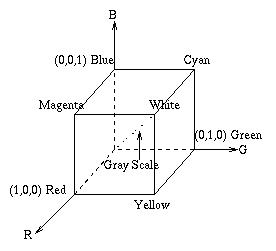
\includegraphics[width=0.55\linewidth]{media/rgb.jpg}
    \caption{\textbf{Az RGB színmodell.}} 
    \label{fig:rgb}
    \end{center}
\end{figure}

\bibliographystyle{unsrt}
\bibliography{references}

\end{document}


 

